% CS 418: Intro to Data Science — Worksheet 19 (19-week10-day1)
% Week 10, Monday 2026-10-26
% Compile with: latexmk -pdf worksheet.tex

\documentclass[11pt]{article}

% ── Packages ──────────────────────────────────────────────────────────────────
\usepackage[margin=0.65in, headheight=14pt]{geometry}
\usepackage{amsmath, amssymb}
\usepackage{ragged2e}
% Never break a word across lines, including at hyphens ("Sans-Serif").
\hyphenpenalty=10000
\exhyphenpenalty=10000
\usepackage{enumitem}
\usepackage{booktabs}
\usepackage{graphicx}
\usepackage{hyperref}
\usepackage{xcolor}
\usepackage{fancyhdr}
\usepackage{mdframed}
\usepackage{array}
\usepackage{tabularx}
\usepackage{tikz}

% ── Page style ────────────────────────────────────────────────────────────────
\pagestyle{fancy}
\fancyhf{}
\lhead{\textbf{CS 418: Intro to Data Science}}
\rhead{UIC, Fall 2026}
\cfoot{\thepage}
\renewcommand{\headrulewidth}{1pt}
\setlength{\headheight}{12pt}
\setlength{\headsep}{0.4cm}

% ── Hyperlinks ────────────────────────────────────────────────────────────────
\hypersetup{colorlinks=false, hidelinks}

% ── Convenience environments ──────────────────────────────────────────────────
% Usage: \fixedblock[height]{content} — a full-width block exactly that tall.
\newcommand{\fixedblock}[2][5.7cm]{\noindent\begin{minipage}[t][#1][t]{\linewidth}\raggedright #2\end{minipage}\par}

% Usage: \choicerow{task}{choice} — one row of a circle-one table (checkpoints 1 and 4), with space for the answer column.
\newcommand{\choicerow}[2]{\small #1 & \small #2 & \\ \hline}

% Usage: \merge{x1}{h1}{x2}{h2}{h} — one dendrogram merge: children at x1 and x2 (already at heights h1 and h2) joined by a bar at height h, inside a tikzpicture.
\newcommand{\merge}[5]{\draw[line width=0.9pt] (#1,#2) -- (#1,#5) -- (#3,#5) -- (#3,#4);}

% Usage: \dbpoint{x}{y}{label} — one labeled point on the checkpoint 7 grid, inside a tikzpicture.
\newcommand{\dbpoint}[3]{%
  \fill (#1,#2) circle (0.09);
  \node[font=\footnotesize, anchor=south west, inner sep=1.5pt] at (#1,#2) {#3};%
}

% ══════════════════════════════════════════════════════════════════════════════
\begin{document}
\RaggedRight

% ── Title block: topic left, info box right ───────────────────────────────────
\noindent
\begin{minipage}[t]{0.55\textwidth}
  \vspace{0pt}
  {\LARGE \textbf{Worksheet \#\,19}} \\[0.18em]
  {\large \textit{Week 10, Day 1: Clustering}}
\end{minipage}
\hfill
\begin{minipage}[t]{0.40\textwidth}
  \vspace{0pt}
  \small
  Name: \underline{\hspace{4.5cm}} \\[0.35em]
  NetID: \underline{\hspace{4.3cm}} \\[0.35em]
  Date: \underline{\hspace{4.4cm}} \\
\end{minipage}

\vspace{0.6em}
\noindent\rule{\linewidth}{0.6pt}
\vspace{0.1em}

\noindent\underline{\textbf{Guided checkpoints}}\\[0.2em]
\noindent{\small For full credit, fill in the checkpoints. If you skip a checkpoint, you must include your own notes for full credit.}
\vspace{0.8em}

% ── 1. Supervised or unsupervised? ───────────────────────────────────────────
\fixedblock[0.19\textheight]{%
\noindent\textbf{1. Supervised or Unsupervised?}\\[0.18em]
\noindent Circle \textbf{S} (supervised) or \textbf{U} (unsupervised) for each task. If it is supervised, name the target variable.

\vspace{0.5em}
\noindent
{\setlength{\tabcolsep}{4pt}%
\renewcommand{\arraystretch}{1.3}%
\begin{tabularx}{\linewidth}{|>{\raggedright\arraybackslash}X|c|p{4.2cm}|}
  \hline
  \small Task & \small Type & \small Target (if supervised) \\ \hline
  \choicerow{Predict a Cook County condo's sale price from its square footage and neighborhood.}{S \enspace / \enspace U}
  \choicerow{Group CTA stations whose weekday ridership looks alike.}{S \enspace / \enspace U}
  \choicerow{Predict a penguin's species from its bill and flipper measurements.}{S \enspace / \enspace U}
  \choicerow{Sort 4,500 movie reviews into groups without looking at their labels.}{S \enspace / \enspace U}
  \choicerow{Flag condo sales whose prices look unusual next to similar sales.}{S \enspace / \enspace U}
\end{tabularx}}
}

\vfill

% ── 2. Draw a bad start / 3. Same data, different answer ─────────────────────
% Checkpoint 2: e.g., two starting centroids in one blob and one between the other two; k-means then splits a blob and merges the other two, like Run A.
% Checkpoint 3: SSE values match the slides' kmeans-restarts figures (Run A 206.1, Run B 157.8).
\fixedblock[0.25\textheight]{%
\noindent
\begin{minipage}[t]{0.48\linewidth}
  \vspace{0pt}\raggedright
  \textbf{2. Draw a Bad Start}\\[0.18em]
  Draw three starting centroids ($\times$) that would leave k-means ($K = 3$) stuck in a bad clustering. Then circle the three clusters it would end with.

  \vspace{0.4em}
  \begin{tikzpicture}[scale=1.15]
    \draw[gray!70] (0,0) rectangle (5.8,4.4);
    \foreach \p in {(0.8,1.0), (1.2,1.5), (1.5,0.9), (1.0,0.6), (1.6,1.3),
                    (4.2,1.0), (4.6,1.5), (5.0,0.9), (4.5,0.6), (4.9,1.3),
                    (2.5,3.4), (2.9,3.9), (3.3,3.5), (2.7,3.0), (3.2,3.1)}
      \fill \p circle (0.06);
  \end{tikzpicture}
\end{minipage}
\hfill
\begin{minipage}[t]{0.48\linewidth}
  \vspace{0pt}\raggedright
  \textbf{3. Same Data, Different Answer}\\[0.18em]
  Two runs of k-means on the same penguins, both with $K = 3$, give different clusterings: Run A has SSE 206.1 and Run B has SSE 157.8. Which run would you keep, and why can the same algorithm give two different answers?

  \vspace{4.2em}
  Name two ways to choose better initial centroids. What can go wrong with one of them?
\end{minipage}
}

\vfill

% ── 4. Partitional or hierarchical? ──────────────────────────────────────────
% Key: H, P, H, P.
\fixedblock[0.18\textheight]{%
\noindent\textbf{4. Partitional or Hierarchical?}\\[0.18em]
\noindent Circle \textbf{P} (partitional) or \textbf{H} (hierarchical) for the clustering each task needs, and say why in a few words.

\vspace{0.5em}
\noindent
{\setlength{\tabcolsep}{4pt}%
\renewcommand{\arraystretch}{1.3}%
\begin{tabularx}{\linewidth}{|>{\raggedright\arraybackslash}X|c|p{6.4cm}|}
  \hline
  \small Task & \small Type & \small Why? \\ \hline
  \choicerow{Build a family tree of penguin species and their relatives.}{P \enspace / \enspace H}
  \choicerow{Split a delivery area into 5 driver zones.}{P \enspace / \enspace H}
  \choicerow{Organize songs into genres, subgenres, and sub-subgenres.}{P \enspace / \enspace H}
  \choicerow{Group customers into 3 segments for a mailing.}{P \enspace / \enspace H}
\end{tabularx}}
}

\newpage

% ── 5. Read a dendrogram ─────────────────────────────────────────────────────
% Merges: 1+2 (1), 4+5 (1.5), 6+7 (2), 3+(45) (2.5), 8+(67) (3), (12)+(345) (5), everything (7).
% Key: 1 and 2; a cut between 3 and 5 gives {1,2}, {3,4,5}, {6,7,8}; a cut at 2.25 gives 5 clusters.
\fixedblock[0.20\textheight]{%
\noindent\textbf{5. Read a Dendrogram}\\[0.18em]
\noindent
\begin{minipage}[t]{0.50\linewidth}
  \vspace{0pt}
  \begin{tikzpicture}[x=0.85cm, y=0.42cm]
    \foreach \y in {1,...,8} \draw[gray!35] (0.4,\y) -- (8.6,\y);
    \draw (0.4,0) -- (0.4,8.3);
    \foreach \y in {0,2,...,8} \node[font=\footnotesize, anchor=east] at (0.4,\y) {\y};
    \node[font=\footnotesize, rotate=90] at (-0.4,4) {merge distance};
    \foreach \x in {1,...,8} \node[font=\small, anchor=north] at (\x,-0.1) {\x};
    \merge{1}{0}{2}{0}{1}
    \merge{4}{0}{5}{0}{1.5}
    \merge{6}{0}{7}{0}{2}
    \merge{3}{0}{4.5}{1.5}{2.5}
    \merge{6.5}{2}{8}{0}{3}
    \merge{1.5}{1}{3.75}{2.5}{5}
    \merge{2.625}{5}{7.25}{3}{7}
  \end{tikzpicture}
\end{minipage}
\hfill
\begin{minipage}[t]{0.46\linewidth}
  \vspace{0pt}
  Which two points are most similar? \underline{\hspace{1.5cm}}

  \vspace{1.2em}
  Draw a horizontal line that cuts the tree into 3 clusters. List them:

  \vspace{1.8em}
  How many clusters does a cut at height 2.25 make? \underline{\hspace{1cm}}
\end{minipage}
}

\vfill

% ── 6. Build a dendrogram ────────────────────────────────────────────────────
% Single link merges AB (2), DE (3), C into DE (4), then everything (5).
% Complete link merges AB (2), DE (3), C into AB (6), then everything (10).
\fixedblock[0.28\textheight]{%
\noindent\textbf{6. Build a Dendrogram}\\[0.18em]
\noindent Use \textbf{single link} (MIN) on the distances below. Draw each merge on the axes at the height where it happens. Then draw a horizontal line that cuts the tree into 2 clusters.

\vspace{0.6em}
\noindent
\begin{minipage}[t]{0.44\linewidth}
  \vspace{0pt}
  {\setlength{\tabcolsep}{5pt}%
  \renewcommand{\arraystretch}{1.3}%
  \begin{tabular}{c|ccccc}
       & A & B & C & D & E \\ \hline
     A & 0 & 2 & 6 & 10 & 9 \\
     B &   & 0 & 5 & 9 & 8 \\
     C &   &   & 0 & 4 & 7 \\
     D &   &   &   & 0 & 3 \\
     E &   &   &   &   & 0 \\
  \end{tabular}}

  \vspace{0.7em}
  The 2 clusters are \underline{\hspace{3.2cm}}

  \vspace{0.7em}
  With \textbf{complete link} (MAX) instead, which cluster does C join, and at what height?
\end{minipage}
\hfill
\begin{minipage}[t]{0.53\linewidth}
  \vspace{0pt}
  \begin{tikzpicture}[x=1.5cm, y=0.34cm]
    \foreach \y in {1,...,10} \draw[gray!35] (0.4,\y) -- (5.6,\y);
    \draw (0.4,0) -- (0.4,10.4);
    \draw (0.4,0) -- (5.6,0);
    \foreach \y in {0,2,...,10} \node[font=\footnotesize, anchor=east] at (0.4,\y) {\y};
    \node[font=\footnotesize, rotate=90] at (-0.05,5) {merge distance};
    \foreach \x/\name in {1/A, 2/B, 3/C, 4/D, 5/E} {
      \fill (\x,0) circle (0.06);
      \node[font=\small, anchor=north] at (\x,-0.1) {\name};
    }
  \end{tikzpicture}
\end{minipage}
}

\vfill

% ── 7. Core, border, noise ───────────────────────────────────────────────────
% With Eps 1.5 and MinPts 4: core A B C D H I; border E G J K; noise F L.
% F is within Eps of E, but E is only a border point, so F stays noise.
\fixedblock[0.40\textheight]{%
\noindent\textbf{7. Core, Border, Noise}\\[0.18em]
\noindent Run DBSCAN with $Eps = 1.5$ grid squares and $MinPts = 4$, counting the point itself. Use the circle at right to check each neighborhood. Write \textbf{C} (core), \textbf{B} (border), or \textbf{N} (noise) next to each point. Then draw a loop around each cluster.

\vspace{0.6em}
\noindent
\begin{tikzpicture}[scale=0.9]
  \draw[gray!35] (0,0) grid (10,5);
  \dbpoint{1}{1}{A}
  \dbpoint{2}{1}{B}
  \dbpoint{1}{2}{C}
  \dbpoint{2}{2}{D}
  \dbpoint{3}{3}{E}
  \dbpoint{4}{4}{F}
  \dbpoint{7}{1}{G}
  \dbpoint{7}{2}{H}
  \dbpoint{8}{2}{I}
  \dbpoint{7}{3}{J}
  \dbpoint{9}{3}{K}
  \dbpoint{4}{1}{L}
  % Reference circle of radius Eps, off to the side of the points.
  \draw[dashed] (12.2,2.5) circle (1.5);
  \fill (12.2,2.5) circle (0.05);
  \draw[->] (12.2,2.5) -- node[font=\footnotesize, above] {$Eps$} (13.7,2.5);
\end{tikzpicture}

\vspace{0.6em}
How many clusters did DBSCAN find? \underline{\hspace{1.5cm}}

\vspace{0.6em}
F is only about 1.4 squares from E, and E is in a cluster. Why isn't F in that cluster?
}

\end{document}
